\documentclass[11pt,a4paper]{article}
\usepackage[utf8]{inputenc}
\usepackage[french]{babel}
\usepackage[T1]{fontenc}

\usepackage{amsmath}
\usepackage{amsfonts}
\usepackage{amssymb}

\newcommand{\NomAuteur}{Fabrice BOISSIER}
\newcommand{\TitreMatiere}{Algo et Structure de Données 1}
\newcommand{\NomUniv}{EPITA - Bachelor Cyber Sécurité}
\newcommand{\NiveauUniv}{CYBER1}
\newcommand{\NumGroupe}{CYBER1}
\newcommand{\AnneeUniv}{2022-2023}
\newcommand{\DateExam}{18 avril 2023}
\newcommand{\TypeExam}{Rattrapage}
\newcommand{\TitreExam}{\TitreMatiere}
\newcommand{\DureeExam}{1h30}
\newcommand{\MyWaterMark}{\AnneeUniv} % Watermark de protection

% Ajout de mes classes & definitions
\usepackage{MetalExam} % Appelle un .sty

% "Tableau" et pas "Table"
\addto\captionsfrench{\def\tablename{Tableau}}

%%%%%%%%%%%%%%%%%%%%%%%
%Header
%%%%%%%%%%%%%%%%%%%%%%%
\lhead{\TypeExam}							%Gauche Haut
\chead{\NomUniv}							%Centre Haut
\rhead{\NumGroupe}							%Droite Haut
\lfoot{\DateExam}							%Gauche Bas
\cfoot{\thepage{} / \pageref*{LastPage}}	%Centre Bas
\rfoot{\texttt{\TitreMatiere}}				%Droite Bas

%%%%%

\usepackage{tabularx}

\newlength{\LabelWidth}%
%\setlength{\LabelWidth}{1.3in}%
\setlength{\LabelWidth}{1cm}%
%\settowidth{\LabelWidth}{Employee E-mail:}%  Specify the widest text here.

% Optional first parameter here specifies the alignment of
% the text within the \makebox.  Default is [l] for left
% alignment. Other options are [r] and [c] for right and center
\newcommand*{\AdjustSize}[2][l]{\makebox[\LabelWidth][#1]{#2}}%


\definecolor{mGreen}{rgb}{0,0.6,0}
\definecolor{mGray}{rgb}{0.5,0.5,0.5}
\definecolor{mPurple}{rgb}{0.58,0,0.82}
\definecolor{backgroundColour}{rgb}{0.95,0.95,0.92}

\lstdefinestyle{CStyle}{
    backgroundcolor=\color{backgroundColour},
    commentstyle=\color{mGreen},
    keywordstyle=\color{magenta},
    numberstyle=\tiny\color{mGray},
    stringstyle=\color{mPurple},
    basicstyle=\footnotesize,
    breakatwhitespace=false,
    breaklines=true,
    captionpos=b,
    keepspaces=true,
    numbers=left,
    numbersep=5pt,
    showspaces=false,
    showstringspaces=false,
    showtabs=false,
    tabsize=2,
    language=C
}


\hyphenation{op-tical net-works SIGKILL}


\begin{document}

%\MakeExamTitleDuree     % Pour afficher la duree
\MakeExamTitle                   % Ne pas afficher la duree

%% \MakeStudentName    %% A reutiliser sur chaque nouvelle page

\bigskip
%\bigskip

Vous devez respecter les consignes suivantes, sous peine de 0 :

\begin{enumerate}[label=\Roman*)]
\item Lisez le sujet en entier avec attention
\item Répondez sur le sujet
\item Ne détachez pas les agrafes du sujet
\item \'Ecrivez lisiblement vos réponses (si nécessaire en majuscules)
\item Vous devez écrire dans le langage algorithmique classique ou en C (donc pas de Python ou autre)
\item Ne trichez pas
\end{enumerate}

%\bigskip

\vfillFirst

% Questions cours
\section{Questions (5 points)}

%\subsection{(1 point) \'Ecrivez l'état d'une file après avoir effectué ces opérations (la file est considérée comme initialement vide) : }
\subsection{(1 point) \'Ecrivez l'état d'une file après avoir effectué ces opérations (la file est considérée comme initialement vide), puis, indiquez quel élément sortira de la file lors du prochain \og dequeue \fg{}, ainsi que celui qui sortira en dernier : }

\bigskip

\begin{center}

\begin{large}
enfiler 1, enfiler 3, défiler, enfiler 4, enfiler 5, défiler, défiler, enfiler 6, enfiler 2, défiler, enfiler 1
\end{large}

%\bigskip

\begin{figure}[ht!]
\centering
\centerline{  %%% CENTRAGE HORIZONTAL
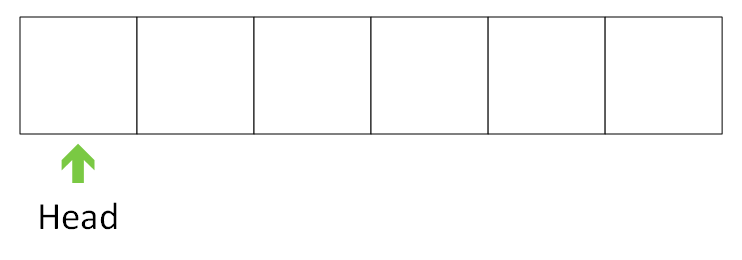
\includegraphics[scale=1]{img/empty_head_2.png}
%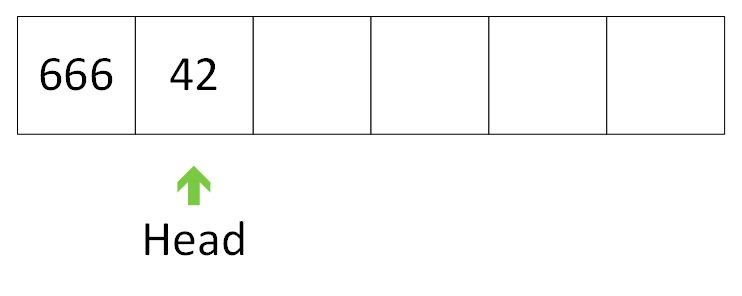
\includegraphics[scale=1,left]{img/2_elts.png}
}
%\caption{File A}
%\label{figure:1-S1-ModeleWI}
\end{figure}

%\end{center}

%\bigskip
\vspace*{-0.75cm}

%%%%%%%%%%%%%%%%%%%%%%%%%%%%%%%%%%%%%%%%%%%%%%%%%%%%%%%%%%%%%%%%%%%%%%%

%\subsection{(1 point) Quel élément sortira de la file lors du prochain \og dequeue \fg{} ? Quel élément sortira en dernier de la file ? }

%\bigskip
%\bigskip

%\begin{center}
\begin{table}[ht!]
%  \centering
  \begin{minipage}{0.50\textwidth}

Prochain élément qui sortira :

  \end{minipage}
  \hfillx
  \begin{minipage}{0.50\textwidth}

Dernier élément qui sortira :

  \end{minipage}
\end{table}
\end{center}

\bigskip

%%%%%%%%%%%%%%%%%%%%%%%%%%%%%%%%%%%%%%%%%%%%%%%%%%%%%%%%%%%%%%%%%%%%%%%
%%%%%%%%%%%%%%%%%%%%%%%%%%%%%%%%%%%%%%%%%%%%%%%%%%%%%%%%%%%%%%%%%%%%%%%

%\subsection{(1 point) \'Ecrivez l'état d'une pile après avoir effectué ces opérations (la pile est considérée comme initialement vide) : }
\subsection{(1 point) \'Ecrivez l'état d'une pile après avoir effectué ces opérations (la pile est considérée comme initialement vide), puis, indiquez quel élément sortira de la pile lors du prochain \og pop \fg{}, ainsi que celui qui sortira en dernier : }

\bigskip

\begin{center}

\begin{large}
empiler 1, empiler 3, dépiler, empiler 4, empiler 5, dépiler, dépiler, empiler 6, empiler 2, dépiler, empiler 1
\end{large}

%\bigskip

\begin{figure}[ht!]
\centering
\centerline{  %%% CENTRAGE HORIZONTAL
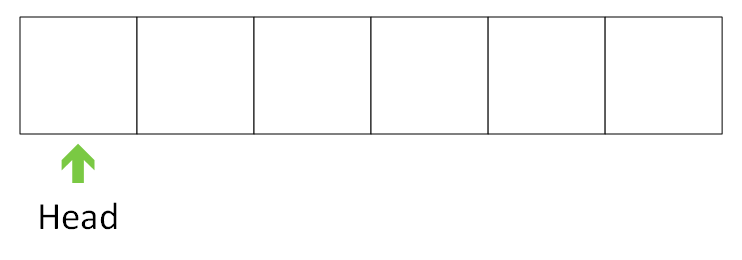
\includegraphics[scale=1]{img/empty_head_2.png}
%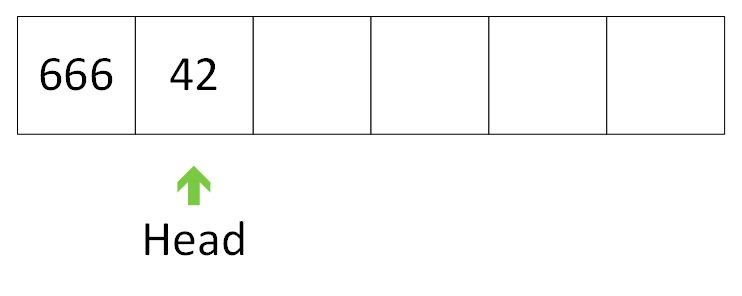
\includegraphics[scale=1,left]{img/2_elts.png}
}
%\caption{File A}
%\label{figure:1-S1-ModeleWI}
\end{figure}

%\end{center}

%\bigskip
\vspace*{-0.75cm}

%%%%%%%%%%%%%%%%%%%%%%%%%%%%%%%%%%%%%%%%%%%%%%%%%%%%%%%%%%%%%%%%%%%%%%%

%\subsection{(1 point) Quel élément sortira de la pile lors du prochain \og pop \fg{} ? Quel élément sortira en dernier de la pile ? }

%\bigskip
%\bigskip

%\begin{center}
\begin{table}[ht!]
%  \centering
  \begin{minipage}{0.50\textwidth}

Prochain élément qui sortira :

  \end{minipage}
  \hfillx
  \begin{minipage}{0.50\textwidth}

Dernier élément qui sortira :

  \end{minipage}
\end{table}
\end{center}

\bigskip
\bigskip


%%%%%%%%%%%%%%%%%%%%%%%%%%%%%%%%%%%%%%%%%%%%%%%%%%%%%%%%%%%%%%%%%%%%%%%

\vfillLast

\clearpage

\subsection{(3 points) En admettant que l'on dispose d'une pile et que l'on insère les données \og 1 2 3 4 5 6 \fg{} dans cet ordre exclusivement, décrivez les scénarios permettant d'obtenir les sorties suivantes : }
%%% PREFERER CE TEXTE :
%\subsection{(3 points) En admettant que l'on dispose d'une pile vide et que les éléments \og 1 2 3 4 5 6 \fg{} arrivent en entrée dans cet ordre exclusivement, décrivez les scénarios permettant d'obtenir les sorties suivantes : }

%\vfillFirst

%\bigskip
\medskip

\begin{center}
\noindent \textit{exemple : pour \og A B C \fg{} en entrée, on peut obtenir \og B C A \fg{} en sortie en faisant : \linebreak
\og push A \fg, \og push B \fg, \og pop \fg, \og push C \fg, \og pop \fg, \og pop \fg }

\noindent \textit{On a bien inséré A, puis B, puis C, mais l'ordre de sortie est différent suivant les \og pop \fg}
\end{center}

\medskip

%\vfillLast


\begin{center}

\begin{large}
1, 2, 3, 6, 5, 4
\end{large}

\begin{center}
\GrilleReponseN{6}
% push 1, pop, push 2, pop, push 3, pop, push 4, push 5, push 6, pop, pop, pop
\end{center}


\begin{large}
3, 2, 4, 5, 1, 6
\end{large}

\begin{center}
\GrilleReponseN{6}
% push 1, push 2, push 3, pop, pop, push 4, pop, push 5, pop, pop, push 6, pop
\end{center}


\begin{large}
2, 3, 5, 4, 6, 1
\end{large}

\begin{center}
\GrilleReponseN{6}
% push 1, push 2, pop, push 3, pop, push 4, push 5, pop, pop, push 6, pop, pop
\end{center}

\end{center}

%\vfillLast
\clearpage

%%%%%%%%%%%%%%%%%%%%%%%%%%%%%%%%%%%%%%%%%%%%%%%%%%%%%%%%%%%%%%%%%%%%%%%%%%%%%%%%%%%%
\section{Algorithmes (15 points)}


\subsection{(1,5 point) \'Ecrivez une structure de données \og \textit{my\_stack\_p} \fg{} pouvant servir de pile (à base de pointeurs ou de tableaux) }

\bigskip

\begin{center}
\GrilleReponseN{10}
\end{center}

\bigskip


\subsection{(1,5 point) \'Ecrivez une structure de données \og \textit{my\_queue\_t} \fg{} pouvant servir de file (à base de pointeurs ou de tableaux) }

\bigskip

\begin{center}
\GrilleReponseN{10}
\end{center}



\newpage

\subsection{(3 points) \'Ecrivez une fonction \og \textit{push} \fg{} pouvant servir à empiler un élément dans votre précédente structure \og \textit{my\_stack\_p} \fg{} }

\bigskip

\begin{center}
%%\LigneReponseQuarante
%\LigneReponseTrente
%\LigneReponseCinq
%\LigneReponseTrois

\GrilleReponseN{24}
\end{center}

\newpage

\subsection{(3 points) \'Ecrivez une fonction \og \textit{pop} \fg{} pouvant servir à dépiler un élément dans votre précédente structure \og \textit{my\_stack\_p} \fg{} }

\bigskip

\begin{center}
\GrilleReponseN{24}
\end{center}

\bigskip



\newpage

\subsection{(3 points) \'Ecrivez une fonction \og \textit{enqueue} \fg{} pouvant servir à enfiler un élément dans votre précédente structure \og \textit{my\_queue\_t} \fg{} }

\bigskip

\begin{center}

\GrilleReponseN{24}
\end{center}

\newpage

\subsection{(3 points) \'Ecrivez une fonction \og \textit{dequeue} \fg{} pouvant servir à défiler un élément dans votre précédente structure \og \textit{my\_queue\_t} \fg{} }

\bigskip

\begin{center}
\GrilleReponseN{24}
\end{center}

\bigskip

%%%%%%%%%%%%%%%%%%%%%%%%%%%%%%%%%%%%%%%%%%%%%%%%%%%%%%%%%%%%%

\clearpage


%\thispagestyle{empty}

\vfillFirst

\begin{center}

\begin{LARGE}
\textbf{RATTRAPAGE ALGORITHMIQUE ET STRUCTURES DE DONN\'EES 1}
\end{LARGE}

\end{center}

\vfillLast

\end{document}
